% Chapter 2

\chapter{Desarrollo e implementaci\'on} % Main chapter title

\label{Chapter4} % For referencing the chapter elsewhere, use \ref{Chapter1} 

%----------------------------------------------------------------------------------------

% Define some commands to keep the formatting separated from the content 

%----------------------------------------------------------------------------------------
En este cap\'itulo se describa la forma de implementaci\'on de la solici\'on
propuesta, as\'i como tambi\'en se describen, lo m\'as detalladamente posible
los m\'etodos, t\'ecnicas y resoluciones aplicadas en dicha implementaci\'on.

\section{Dise\~no estructural}

\begin{figure}[th]
    \centering
    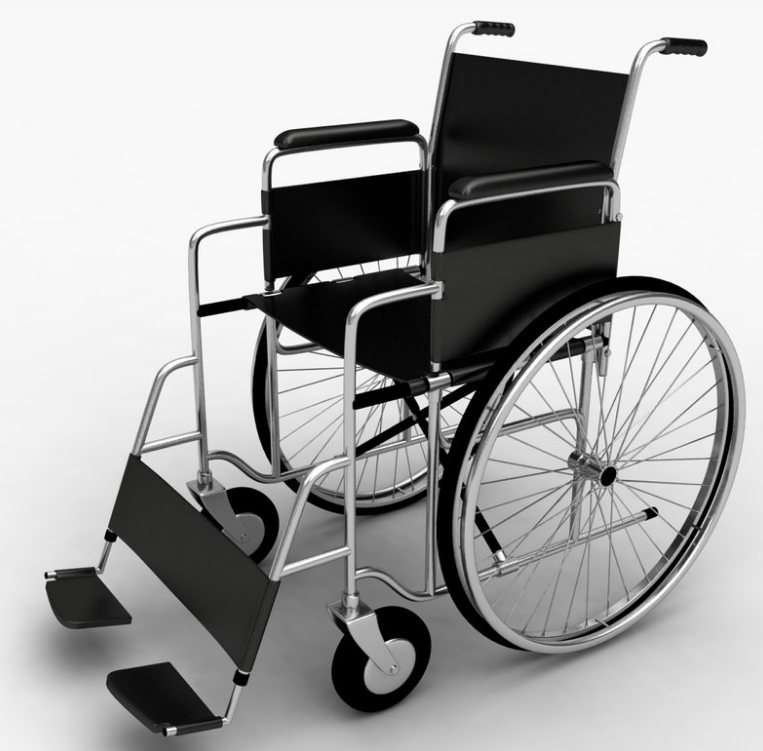
\includegraphics[width=.5\textwidth]{Figures/wheelchair.png}
    \decoRule
    \caption{Modelo de silla, base de soluci\'on}
    \label{fig:wheelchair}
\end{figure}

Como se mencion\'o en el cap\'itulo anterior la propuesta indica que se
ampliar\'an las caracter\'isticas de una silla de rueda tradicional a las de una
silla de ruedas \emph{smart}, por lo que, como ya se indic\'o, la base del
proyecto es como tal una silla de ruedas tradicional (fig.\ref{fig:wheelchair}).
El modelo elegido corresponde al m\'as comunmente utilizado en nuestro mercado
(ver cap. \ref{Chapter2}), los sistemas propuestos como parte de la soluci\'on
ser\'an f\'isicamente acoplados a este modelo y la descripci\'on de este
procedimiento es detallada a lo largo de esta secci\'on.

\subsection{Joystick de interfaz}
\begin{figure}[th]
    \centering
    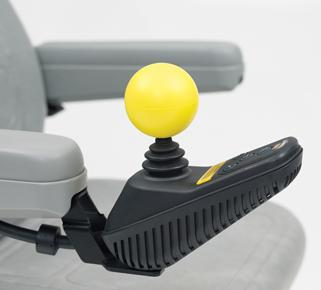
\includegraphics[width=.4\textwidth]{Figures/joystick.jpg}
    \decoRule
    \caption{Interfaz de usuario incrustada en reposabrazos}
    \label{fig:joy}
\end{figure}

Este dispositivo, tiene una gran versatilidad, dada su construcci\'on y que, de
hecho es desarrollado con el prop\'osito en mente de que sea integrado a una
soluci\'on como la nuestra, tiene la preparaci\'on necesaria para montarlo en
nuestro producto final. Seg\'un las observaciones registradas en la
introducci\'on (ref.\ref{implicaciones}) la mejor posici\'on para este
aditamente es en el reposabrazos, por lo que  se posicionar\'a ah\' valiendonos
\'unicamente de un mecanismo de fijaci\'on mec\'anico (tornillo).
Fig.\ref{fig:joy}.

\subsection{M\'odulo de control}

La composici\'on detallada de este m\'odulo se describe en secciones posteriores
del presente, sin embargo las dimensiones y posicionamiento f\'isico del mismo
es tratada a continuaci\'on.

\subsubsection{Dimensiones}

\begin{figure}[th]
\centering
\begin{minipage}{.5\textwidth}
  \centering
  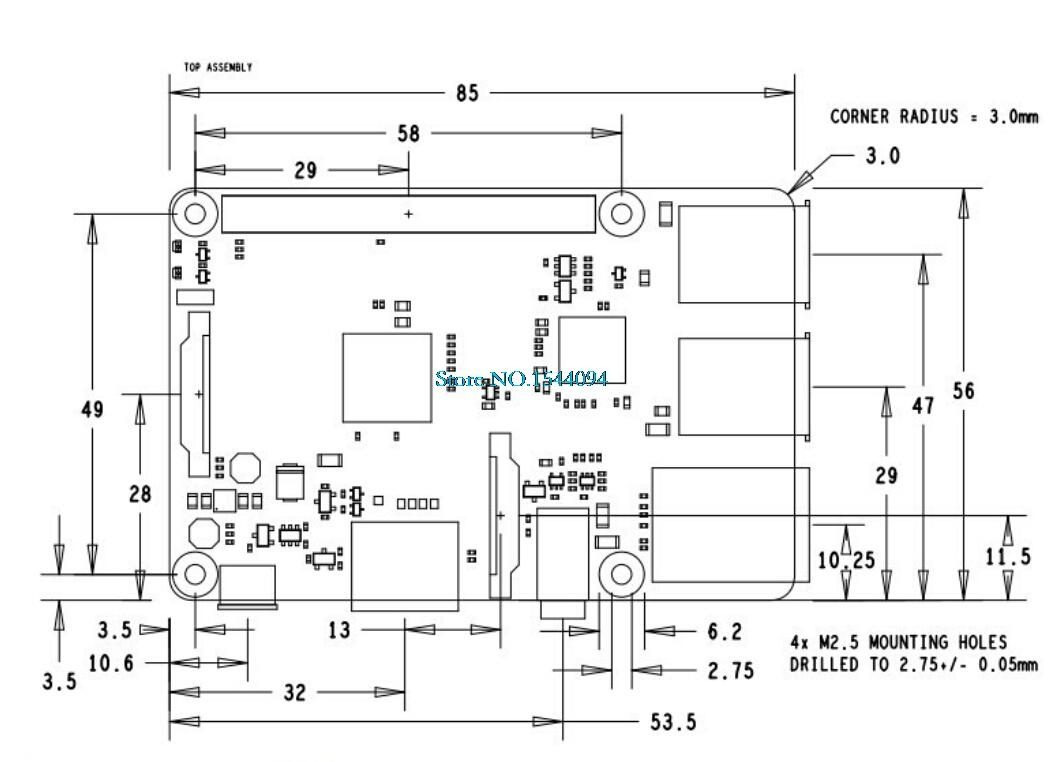
\includegraphics[width=\linewidth]{Figures/rasp_dimensions.jpeg}
  \captionof{figure}{Raspberry pi: dimensiones}
  \label{fig:dimensiones}
\end{minipage}%
\begin{minipage}{.5\textwidth}
  \centering
  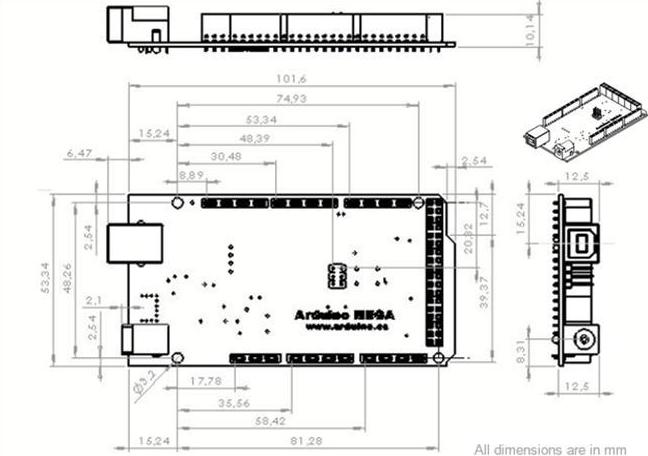
\includegraphics[width=\linewidth]{Figures/ARDUINO-MEGA-2560.jpg}
  \captionof{figure}{Arduino: dimensiones}
\end{minipage}
\end{figure}

Las dimensiones de los componentes principales de este subsistema son indicadas
en la figura \ref{fig:dimensiones}, por otro lado las dimensiones del
controlador de motores son las siguientes: 
\begin{figure}[th]
\centering
\begin{minipage}{.3\textwidth}
  \centering
  \begin{description}
    \item[ancho] $76mm$
    \item[largo] $89mm$
    \item[profundidad] $46mm$
  \end{description}
\end{minipage}%
\begin{minipage}{.7\textwidth}
  \centering
  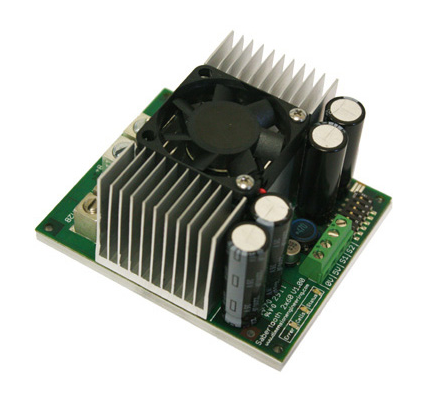
\includegraphics[width=\linewidth]{Figures/motor_driver.png}
  \captionof{figure}{Controlador de motores}
\end{minipage}
\end{figure}

Con los anteriores datos, se propone construir una carcasa pl\'astica en la cual
proteger y ubicar dichos componentes, las dimensiones del \emph{enclousure}
propuesto son las indicadas en la figura \ref{fig:enclousure}.

\begin{figure}
\centering
\begin{minipage}{.3\textwidth}
  \centering
  \begin{description}
    \item[ancho] $200mm$
    \item[largo] $200mm$
    \item[profundidad] $100mm$
  \end{description}
\end{minipage}%
\begin{minipage}{.7\textwidth}
  \centering
  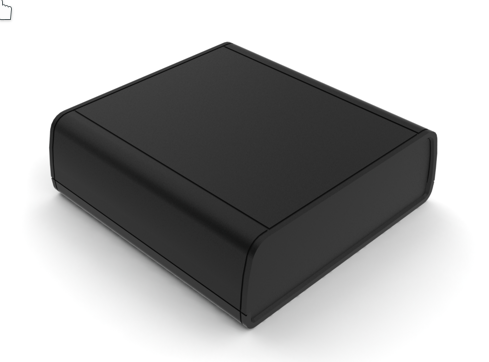
\includegraphics[width=\linewidth]{Figures/enclousure.png}
  \captionof{figure}{\emph{Enclousure} del sisema de control}
  \label{fig:enclousure}
\end{minipage}
\end{figure}

\subsubsection{Posicionamiento}

El m\'odulo de control ser\'a ubicado en la parte inferior del asiento de la
silla, el case ser\'a empotrado mec\'anicamente sobre el sistema de
almacenamiento de energ\'ia.

\subsection{Sistema de potencia}

\begin{figure}
    \centering
    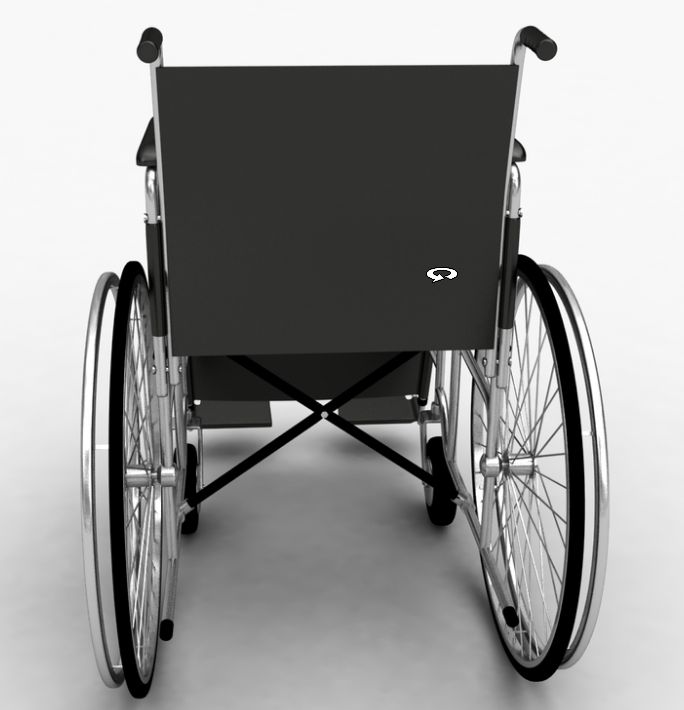
\includegraphics[width=.5\textwidth]{Figures/wheel_back.png}
    \decoRule
    \caption{El sistema de potencia se ubica bajo el asiento}
    \label{fig:back}
\end{figure}
Como est\'a indicado, este se compone tanto de 2 baterias
(fig.\ref{fig:batery}), como de los actuadores principales
(fig.\ref{fig:motor}), estos ser\'an directamente montados en la parte baja de
la silla de ruedas, justo donde se indica en la figura \ref{fig:back}.\\
La transmisi\'on de potencia ser\'a directa entre los motores y cada una de las
ruedas posteriores de la silla, esta forma de transmisi\'on ha demostrado ser
una de las m\'as eficientes, al mismo tiempo que permitir\'a una fabricaci\'on
menos costosa de la soluci\'on final \parencite{motorized}.


\section{Hardware}


El hardware que compone la soluci\'on:
\begin{itemize}
    \item Raspberry pi 3 Model B+
    \item Arduino uno
    \item Controlador de motor Sabertooth Dual 60A
    \item Motor de DC, DG-158A, 2x
    \item Bateria UPG 12v 35AH, 2x
    \item Joystick Controller VR2
    \item Sensor ultras\'onico, 2x
    \item Girosc\'opio y aceler\'ometro, MPU-6050 3 axis

\end{itemize}

\subsection{Esquema de componentes}

\begin{figure}[th]
    \centering
    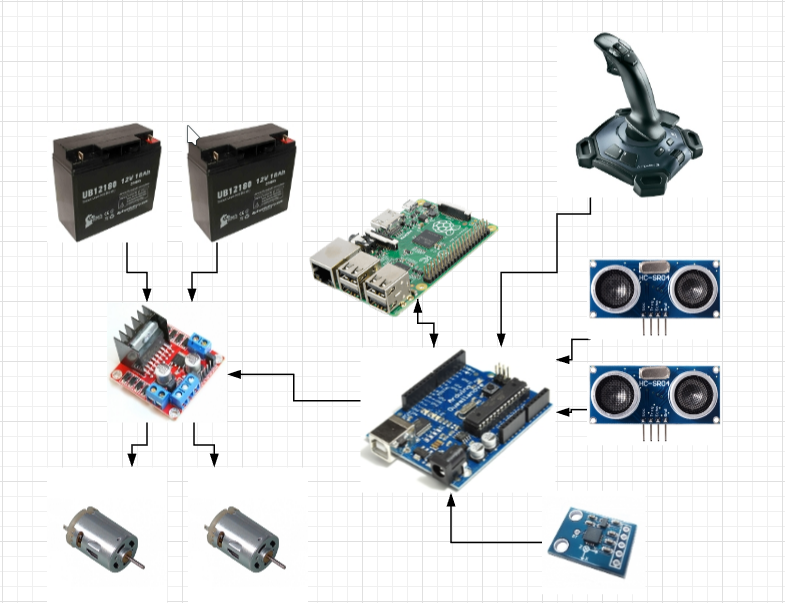
\includegraphics[width=.9\textwidth]{Figures/components.png}
    \decoRule
    \caption{Diagrama esquem\'atico de componentes}
    \label{fig:components}
\end{figure}
Los componentes de hardware estar\'an interconectados seg\'un se muestra en la
figura \ref{fig:components}.

\section{Software}

En la categor\'ia de software, como parte de la propuesta de soluci\'on implica
fabricar una silla de un costo accesible, se optar\'a por el uso de
tecnolog\'ias de uso libre as\'i como de desarrollo hecho a la medida.

